\chapter{Introduction} \label{intro}
The design by the modern world has been shaped by the urge of man to make daily tasks more automated, reducing the man power required. With this increase in automation and robotics comes the desire to create a robotic platform which will be capable of robust and complex movement over varying types of terrain, to aid man in daily task or to assist in dangerous situation (such as firefighters rushing into a burning building). With this come the question of how the platform should move to reach the desired complex movement from it, with the answer being legged locomotion. Legged robotics is by far the most optimal method for locomotion over land as it allows for navigation on rugged terrain along with the capability of rapid agile maneuvers.

Past literature has produced a number of walking platforms, which are in general slow moving making them less piratical \cite{Asimo-2018}. A platform is thus needed which is agile and capable of robust movement, in recent times a few such platform were developed such as the Atlas \cite{Atlas-2019}. These systems and their desired tasks are complex and very non-linear, resulting in designing controllers to become a difficult task.

\begin{figure}[!ht]
    \centering
    \begin{subfigure}[b]{0.4\textwidth}
        \centering
        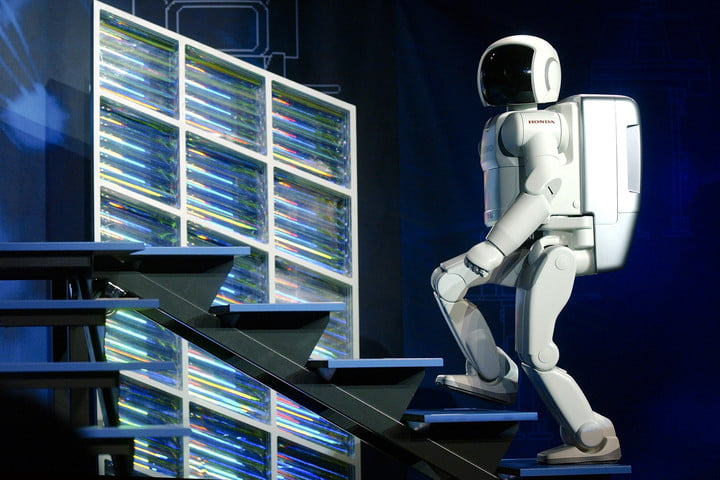
\includegraphics[width=1\linewidth]{figs/asimo.png}
        \caption{Asimo \cite{Asimo-2018}.}
    \end{subfigure} 
    \hfill
    \begin{subfigure}[b]{0.4\textwidth}
        \centering
        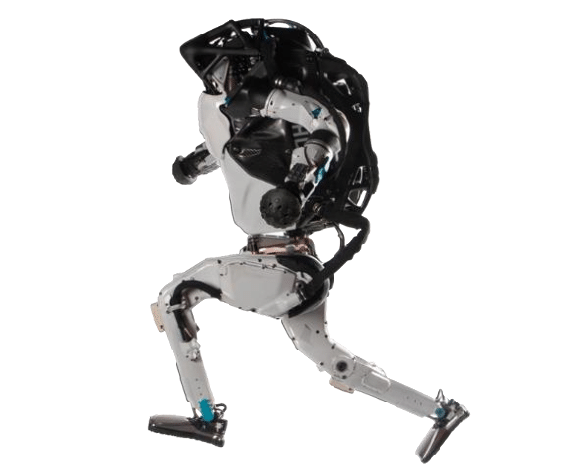
\includegraphics[width=\linewidth]{figs/altals.png}
        \caption{Atlas \cite{Atlas-2019}.}
    \end{subfigure}
    \caption{Two examples of well known walking platforms that have been produced by past literature.}
    \label{fig:linear_sim}
\end{figure}

\section{Motivation and Background to the Study}
Any state-of-the-art robotic platform is vastly inferior in legged locomotion compared to those performed in nature. Legged locomotion in nature comes effortlessly while allowing for high agile movements, not even a current, state-of-the-art, platform like the Atlas \cite{Atlas-2019} (which is capable of running, rolling, crouching and even parkour) can compare to the agile movements in nature. With all these advances in robotics, walking is still considered a complex and unsolved task, that is why preachers apply assumptions such as, massless legs \cite{Kamimura-2018}\cite{Gan-2018}, infinite friction \cite{Kamimura-2018}\cite{Xi-2016} and simplified and reduced order models \cite{Reher-2019}, in order to make the task easier to solve and design controllers for.

In this research trajectory optimisation will be used to generate a path for the robot and then controller will be designed inspired by the trajectory optimisation. Trajectory optimisation has produced research papers in the past \cite{Baleka-2020}\cite{Beck-2009}, and from these paperers it was clear that trajectory inspired control leads to robust and agile movements. 

\section{Research Questions}
words

\section{Scope and Limitations}
asd

\section{Plan of Development}
asd


